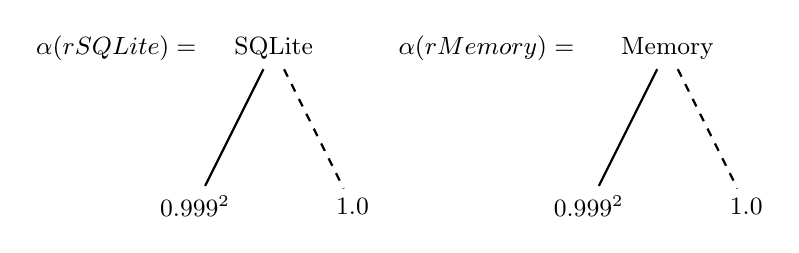
\begin{tikzpicture}[thick]
\centering
\small
\node[draw=none](alphaSqlite) at (-1,2) {$\alpha(rSQLite)=$};
\node(sqlite) at (1,2) {SQLite};
\node[rectangle, draw=none](rSqlite) at (0,0) {$0.999^2$};
\node[rectangle, draw=none](!rSqlite) at (2,0) {$1.0$};
\draw[thick] (sqlite) -- (rSqlite);
\draw[thick, dashed] (sqlite) -- (!rSqlite);

\node(memory) at (6,2) {Memory};
\node[draw=none](alphaMemory) at (3.7,2) {$\alpha(rMemory)=$};
\node[rectangle, draw=none](rMemory) at (5,0) {$0.999^2$};
\node[rectangle, draw=none](!rMemory) at (7,0) {$1.0$};
\draw[thick] (memory) -- (rMemory);
\draw[thick, dashed] (memory) -- (!rMemory);
\end{tikzpicture}
